\documentclass[fleqn,reqno,10pt]{article}

%========================================
% Packages
%========================================

\usepackage[]{../../helpers/mypackages}
%\usepackage[natbib=true,style=authoryear-comp,backend=bibtex,doi=false,url=false]{biblatex}
%\bibliography{MyRefGlobal}
\bibliography{../../helpers/MyRefGlobal}
\bibliography{paper} 
\usepackage{../../helpers/myenvironments}
\usepackage{../../helpers/mycommands}
\usepackage{todonotes}
\usepackage{subcaption}



%========================================
% Standard Layout
%========================================

% Itemize
\renewcommand{\labelitemi}{\large{$\mathbf{\cdot}$}}    % itemize symbols
\renewcommand{\labelitemii}{\large{$\mathbf{\cdot}$}}
\renewcommand{\labelitemiii}{\large{$\mathbf{\cdot}$}}
\renewcommand{\labelitemiv}{\large{$\mathbf{\cdot}$}}
% Description
\renewcommand{\descriptionlabel}[1]{\hspace\labelsep\textsc{#1}}

% Figure Captions
\usepackage{caption} % use corresponding myfiguresize!
\setlength{\captionmargin}{20pt}
\renewcommand{\captionfont}{\small}
\setlength{\belowcaptionskip}{7pt} % standard is 0pt

%========================================
% Additional layout & commands
%========================================


\renewcommand{\Smixed}{\ensuremath{\mathrm{\mathbf{s}}}}
\renewcommand{\Rmixed}{\ensuremath{\mathrm{\mathbf{r}}}}

% Annotations
\newcommand{\mytodo}[2]{\todo[inline,color=yellow,author=#1]{#2}}
\newcommand{\question}[2]{\todo[inline,color=blue,author=#1]{#2}}
\newcommand{\answer}[2]{\todo[inline,color=green,author=#1]{#2}}

\newcommand{\rd}{\acro{rd}} % replicator dynamic
\newcommand{\rmd}{\acro{rmd}} % replicator mutator dynamic
\newcommand{\rdd}{\acro{rdd}} % replicator diffusion dynamic
\newcommand{\RD}{\ensuremath{\mathrm{RD}}} % replicator dynamic
\newcommand{\RDD}{\ensuremath{\mathrm{RDD}}} % replicator diffusion dynamic
\newcommand{\RMD}{\ensuremath{\mathrm{RMD}}} % replicator mutator
                                
\newcommand{\Diff}{\ensuremath{\mathrm{D}}} % Difusion 
\newcommand{\Mutate}{\ensuremath{\mathrm{M}}} % Mutation 

\newcommand{\impairment}{\ensuremath{\alpha}} % impairment
\newcommand{\toler}{\ensuremath{\beta}} % tolerance
\newcommand{\ns}{\ensuremath{n_s}} % number of states

\newcommand{\similarity}{\ensuremath{\mathrm{Sim}}} % similarity function

\doublespacing

\title{Vagueness, Noise, and Signaling}
% \author{Michael Franke \and Jos\'e Pedro Correia}
\date{}

\begin{document}

\maketitle

\begin{abstract}
  Signaling games are popular models for studying the evolution of
  meaning, but typical approaches do not incorporate vagueness as a
  feature of successful signaling.  Complementing recent like-minded
  models, we introduce the replicator diffusion dynamic as a special
  case of the replicator mutator dynamic that combines evolutionary
  pressure on optimal signal use with stochastic noise in the
  processing of similar stimuli. Applying this new dynamic to a
  generalization of Lewis' signaling games, we show that stochastic
  imprecision leads to vague, yet by-and-large communicative efficient
  signal use, and, moreover, that it unifies evolutionary outcomes and helps
  avoid suboptimal categorization.
\end{abstract}

\section{Introduction}
\label{sec:introduction}

Many concepts and expressions are vague. A vague category knows clear
cases that fall under it, clear cases that do not, and also so-called
borderline cases. Borderline cases do not clearly apply, nor do they
clearly not apply, and there may be differences between borderline
cases in terms of how well they represent the category in
question. Vagueness does not seem to dramatically affect the success
of everyday communication, but it is troublesome for some of the most
prominent theories of language and meaning. This is especially so for the logico-semantic tradition of Frege, Russell and the young
Wittgenstein which is challenged by the paradoxes vagueness gives rise
to. 

But there are other intriguing aspects about vagueness. The puzzle
that we are concerned with here is how vagueness could arise and be
maintained in the first place. This is a serious issue for
functionalist accounts that maintain that concepts and linguistic
meanings evolved driven towards efficiency. Since the existence of
unclear borderline cases seems to entail inefficiency of
categorization or communication, the challenge, succinctly put forward
by \citet{Lipman2009:Why-is-Language}, is to explain how vagueness can
persist under evolutionary pressure to be optimally discriminative. We
address \emph{Lipman's problem} as a technical challenge, namely to
find a conceptually sound and mathematically coherent formal model of
the evolution of categorization and language use that yields
by-and-large efficient categorization \emph{and} vagueness.

A number of authors have recently tried to explain why vagueness
evolved as something that is itself useful
\citep[e.g.][]{Jaegherde-Jaegher2003:A-Game-Theoreti,Deemter2009:Utility-and-Lan,BlumeBoard2013:Intentional-Vag}.
Others have argued that vagueness is a natural byproduct of
limitations in information processing or particular learning
strategies
\citep[e.g.][]{FrankeJager2010:Vagueness-Signa,OConnor2013:The-Evolution-o}. This
paper contributes to the latter line of thought. Concretely, we
introduce the replicator diffusion dynamics---a novel variant of the
replicator mutator dynamic---that integrates stochastic noise on the
differential confusability of similar stimuli. The dynamic proposed
here generalizes and complements previous like-minded accounts. We
show that stochastic noise can not only lead to vague, yet relatively
efficient signal use, but also unify evolutionary outcomes and
help avoid suboptimal categorization.

The next section introduces the background against which the work
presented here can be appreciated. Section~\ref{sec:repl-diff-dynam}
introduces the replicator diffusion dynamic and Section~\ref{sec:diffusion-as-special}
elaborates on its relation with the replicator mutator
dynamic. Section~\ref{sec:exploring-rdd} explores the replicator
diffusion dynamic. Section~\ref{sec:discussion} reflects and compares
our approach to others.

\section{Background}
\label{sec:background}

% The view that vagueness is a natural concomitant of cognitive
% limitations of language users has been formalized in a number of ways,
% using evolutionary game theory and certain generalizations of Lewis'
% signaling games \citep{Lewis_1969:Convention}, so called
% \emph{similarity-maximizing games}, or \emph{sim-max games}, for short
% \citep{Jager2007:The-Evolution-o,JagerRooijvan-Rooij2007:Language-Struct}.
% %\citep{FrankeJager2010:Vagueness-Signa,OConnor2013:Evolving-Percep,OConnor2013:The-Evolution-o}.
% Our contribution is best seen in relation to these accounts, as it also
% relies on sim-max games. Let's introduce these first, and then zoom in
% on the problem of vagueness.

\subsection{Sim-max games \& conceptual spaces}

Signaling games, as introduced by \citet{Lewis_1969:Convention}, have
a sender and a receiver. The sender knows the true state of the world,
but the receiver does not. The sender can select a signal, or message,
to reveal to the receiver, who then chooses an act. In Lewis' games,
if the receiver chooses the act that corresponds to the actual state,
the play is a success, otherwise a failure. Certain regular
combinations of sender signaling and receiver reaction make messages
meaningful, in the sense that their use is correlated systematically
to certain states or acts. To investigate the conditions under which
such meaning-generating behavior can evolve is a highly interesting
topic that we are only beginning to fully understand
\citep[e.g.][]{Warneryd1993:Cheap-Talk-Coor,BlumeKim1993:Evolutionary-St,Huttegger2007:Evolution-and-t,Pawlowitsch2008:Why-Evolution-d,Barrett2009:The-Evolution-o,HutteggerSkyrms2010:Evolutionary-Dy,Skyrms2010:Signals}.

Similarity-maximizing (short: sim-max) games are generalizations of
Lewis' games where different states are allowed to be more or less
similar to one another. While Lewis' games treated communicative
success as a matter of black and white, sim-max games allow for a
gradient notion: the more similar the receiver's interpretation is to
the actual state, the better. Signaling games with utility-relevant
similarities in the state space are fairly standard in economics
\citep[e.g.][]{Spence1973:Job-market-sign,CrawfordSobel1982:Strategic-Infor},
but have received particular attention in a more philosophical context
for reasons that will become clear presently
\citep{Jager2007:The-Evolution-o,JagerRooijvan-Rooij2007:Language-Struct,JagerMetzger2011:Voronoi-Languag}.

A sim-max game consists of a set of states $\States$, a set of
messages $\Messgs$ with much fewer messages than states, a prior
probability distribution $\Pr \in \Delta(\States)$ that gives the
occurrence probabilities of states, a similarity metric on states
$\similarity \mycolon \States \times \States \rightarrow \mathds{R}$,
and a utility function $\Utils \mycolon \States \times \States
\rightarrow \mathds{R}$. We identify the receiver's acts with the
states of the world, so that the game is one of guessing the actual
state, so to speak. We also assume that sender's and receiver's
interests are alike, so we only have one utility function. We do not
consider message costs, so utilities only depend on the actual state
and the receiver's response. The utility function should be a
monotonically decreasing function of similarity.

\citet{JagerMetzger2011:Voronoi-Languag} showed that the
evolutionarily stable states of sim-max games are remarkably
systematic. Their results were obtained for games with infinitely many
states in $n$-dimensional Euclidean space $\States \subseteq
\mathds{R}^n$ and a quadratic loss function for utilities
$\Utils(\mystate{1}, \mystate{2}) = - (\mystate{1} -
\mystate{2})^2$. For these games, the evolutionarily stable states are
demonstrably so-called Voronoi languages. Roughly put, a Voronoi
language is a pair of sender and receiver strategies, such that the
sender strategy partitions the state space into convex categories,
while the receiver's interpretations are the central spots in each
category. A subset $X$ of $\mathds{R}^n$ is convex if, informally put,
all points in $X$ are connected via a straight line that lies entirely
in $X$; $X$ has no gaps or dents. For example, if \States is the unit
interval and all states are equiprobable, a Voronoi language with two
messages would have the sender use one message exclusively for all
points in the lower half of the unit interval and another for all
points in the upper half; the receiver's interpretations of messages
are the central points, .25 and .75, in the respective intervals.

This result is interesting, because it demonstrates that signaling can
impose orderly categories on a metric space, without that being the
ulterior purpose of it all. Sender and receiver can be distinct
entities, whose purpose is to communicate effectively about the actual
state. In that case, evolving Voronoi languages would explain why
\emph{linguistic categories} are well-behaved and orderly in the way
they appear to be. More abstractly, sender and receiver can also be
thought of as distinct modules in a single system, where the first
module must discretize the information it is fed by selecting a small
sample of, suggestively, category labels. These are passed to a second
module that tries to decode the original information. In this case,
evolving Voronoi languages would explain why \emph{conceptual
  categories} are well-behaved and orderly in the way that they appear
to be.

Seen in this light, sim-max games may provide a foundation to
approaches in cognitive semantics that rely on the notion of
conceptual spaces.  \citet[][70--77]{Gardenfors2000:Conceptual-Spac},
for example, has prominently argued that natural categories are convex
regions in conceptual space. If the conceptual space has a suitable
metric, convex categories can be derived from a set of prototypes. The
category corresponding to prototype $p$ is the set of points that are
more similar to $p$ than to any other. In this way,
\citet{Gardenfors2000:Conceptual-Spac} argues, an efficient
categorization system can be obtained: storing the prototypes lets us
recover the categories without having to store each category's
extension. However, what is left unexplained, is where the prototypes
come from, and why we would not see just any distribution of
prototypes as an equally efficient classification system. This is
where sim-max games can contribute a principled approach to deriving,
in an independent way, not only convex categories but also
prototypical exemplars belonging to them.


\subsection{Vague signaling in sim-max games}

This outline of an approach to categorization using sim-max games
leaves many problems unaddressed. One of them is that natural
categories for continuously variable stimuli usually do not have
unique, point-valued prototypes and clear category boundaries. We
would like to account for the possibility of such vagueness, in
particular: (i) clear positive examples of a vague category should
show a gradient transition to clear negative examples;
(ii) prototypes should likewise be gradient regions, peaking at the
center of the vague category they represent.

\citet{DouvenDecock2011:Vagueness:-A-Co} show that
\citeauthor{Gardenfors2000:Conceptual-Spac}'s conceptual spaces
approach can be extended to account for the existence of borderline
cases. From the assumption that prototypes are extended, yet convex
regions in conceptual space, a construction algorithm is available
that yields ``collated Voronoi diagrams'' with thick boundaries
representing borderline
regions. \citet{DecockDouven2012:What-is-Graded-} show further how it
is possible to arrive at a gradient transition between categories, by
weighing in the distance of different borderline cases to various
prototypical regions. This accounts for the first of the two
desiderata mentioned above, but still assumes that crisp prototype
regions must be given.

An alternative approach is taken by
\citet{FrankeJager2010:Vagueness-Signa} and
\citet{OConnor2013:The-Evolution-o} who show how the above desiderata
can be met by evolving strategies in sim-max games. The approach we
take here is similar in spirit, but different in relevant detail. We
argue here that \citeauthor{FrankeJager2010:Vagueness-Signa}'s
approach gives rise to problematic predictions under certain
conditions which are avoided in our approach. While
\citeauthor{OConnor2013:The-Evolution-o} gives an agent-level learning
dynamic under which vague signaling arises, we complement the picture
by giving a population-level dynamic that abstracts from the concrete
behavior of signalers. A more in-depth comparison is deferred until
Section~\ref{sec:discussion}. Let us first look into our own proposal
in more detail.


%%%%%%%%%%%%%%%%%%%%%%%%%%%%%%%%%%%%%%%%%%%%%%%%%%
%%%%%%%%%%%%%%%%%%%%%%%%%%%%%%%%%%%%%%%%%%%%%%%%%%

\section{Replicator diffusion dynamic}
\label{sec:repl-diff-dynam}

We introduce a population-level dynamic in which communicatively more
efficient strategies increase in proportion, as usual, but where the
realization of signaling strategies is noisy because of the agents'
inability to sharply distinguish similar states. We call our dynamic
\emph{replicator diffusion dynamic} (\rdd), because it is an extension
of the replicator dynamic (\rd) and a special case of the replicator
mutator dynamic (\rmd).

The formulation of the \rdd given and explored here is in terms of
behavioral strategies, not in terms of mixed strategies. Dynamics on
behavioral strategies assume that agents can adapt
their behavior locally, so to speak, i.e., independently at each
choice point. This greatly reduces the complexity of the dynamic and
simplifies numerical simulations. But it also points towards an
interpretation of the process as cultural evolution, rather than
biological evolution. Signaling strategies are not inherited as a
whole, but adapted piece-meal, e.g., by conditional imitation of
``local'' behavior at a given choice point (more below). Still, the
approach we suggest here is compatible with a formulation in terms of
mixed strategies and an interpretation as biological evolution as
well. In Section~\ref{sec:diffusion-as-special}, we
translate our initial formulation of the \rdd
into one using mixed strategies. Doing so identifies the \rdd as a
special case of the \rmd. For now, let us first focus on the
formulation of the dynamic in terms of behavioral strategies alone.

We begin by recapitulating the \rd in
Section~\ref{sec:repl-dynam-behav}, and introduce the \rdd in
Section~\ref{sec:repl-diff-dynam-1}.
%Section~\ref{sec:repl-mutat-dynam} introduces the \rmd, and
%Section~\ref{sec:diffusion-as-special} shows in what sense the \rdd is
%a special case of the \rmd. Sections~\ref{sec:repl-mutat-dynam} and
%\ref{sec:diffusion-as-special} are conceptually important, but rather
%technical and not strictly necessary to appreciate the main point of
%the paper.

\subsection{Replicator dynamic in behavioral strategies}
\label{sec:repl-dynam-behav}

Fix a signaling game with finite states $\States$, messages $\Messgs$
and acts $\Acts$. Let $\Pr(\cdot) \in \Delta{\States}$ be the prior
distribution over states and $\Util_{\sen,\rec} \mycolon \States
\times \Messgs \times \Acts \rightarrow \mathds{R}$ the sender's and
receiver's utility functions. A behavioral strategy is a function that
maps an agent's choice points to a probability distribution over
available choices. The sender's behavioral strategies are functions
$\Sstrat \in \Delta(\Messgs)^\States$; the receiver's are functions
$\Rstrat \in \Delta(\Acts)^\Messgs$. The expected utility of choices
at each choice point is:
\begin{align*}
  \EU(\messg, \state, \Rstrat) & = \sum_{\act \in \Acts}
  \Rstrat(\act \probbar \messg) \cdot U_\sen(\state, \messg, \act) \\
  \EU(\act, \messg, \Sstrat) & = \sum_{\state \in
    \States} \Pr(\state) \cdot \Sstrat(\messg \probbar \state) \cdot
  U_\rec(\state, \messg, \act) \,.
\end{align*}
The \emph{fitness} of a behavioral strategy at a choice point is the
frequency-weighted average of expected utilities of each choice, given
the opponent's strategy:
\begin{align*}
  \Phi(\state,\Sstrat, \Rstrat) & = \sum_{\messg} \Sstrat(\messg \probbar \state) \cdot
\EU(\messg, \state,\Rstrat) \\
\Phi(\messg,\Sstrat, \Rstrat) & = \sum_{\act} \Rstrat(\act \probbar \messg)
\cdot \EU(\act, \messg,\Sstrat)\,.
\end{align*}
The discrete-time replicator dynamic maps current strategies $\Sstrat$
and $\Rstrat$ to future strategies $\RD(\Sstrat)$ and $\RD(\Rstrat)$
in such a way that changes in frequency are proportional to expected
utilities. For behavioral strategies, the changes take place locally
at each of the agents' choice points:
\begin{align*}
  \RD(\Sstrat)(\messg \probbar \state) & = \frac{\Sstrat(\messg \probbar \state) \cdot
    \EU(\messg, \state,\Rstrat)} {\Phi(\state,\Sstrat, \Rstrat)} \\
    \RD(\Rstrat)(\act \probbar \messg) & = \frac{\Rstrat(\act \probbar \messg) \cdot
    \EU(\act, \messg,\Sstrat)} {\Phi(\messg,\Sstrat, \Rstrat)}  \,.
\end{align*}
The \rd in behavioral strategies describes the most likely path of
development of average behavior in a population
of agents when behavioral adaptations occur independently at each
choice point, e.g., when agents adopt the behavior of another agent
\emph{at a given choice point} if that ``local'' behavior is
``locally'' better than their own (see
\citeauthor{Sandholm2013:Population-Game}
\citeyear{Sandholm2013:Population-Game} for agent-level
interpretations of the replicator dynamics and
\citeauthor{Cressman2003:Evolutionary-Dy}
\citeyear{Cressman2003:Evolutionary-Dy} for applications to extensive
form games and behavioral strategies).


\subsection{Replicator diffusion dynamic in behavioral strategies}
\label{sec:repl-diff-dynam-1}

The replicator diffusion dynamic is a noise-perturbed variant of the
\rd in behavioral strategies. Fix a sim-max game with $\States =
\Acts$ and a confusion matrix $C : \States \times \States$. $C$ is a
row-stochastic matrix, i.e., each row is a probability
distribution. Elements $C_{ij}$ give the probability that $\state_i$
is realized as $\state_j$. The confusability of states affects senders
and receivers alike, but in slightly different ways (see
Figure~\ref{fig:noise-perturbation-of-strategies}). For the sender,
$C_{ij}$ is the probability that the actual state \mystate{i} is
perceived as \mystate{j}. For the receiver, $C_{ij}$ is the
probability that \mystate{j} is the interpretation that is actually
formed when \mystate{i} is the intended interpretation.

\begin{figure}
  \centering

    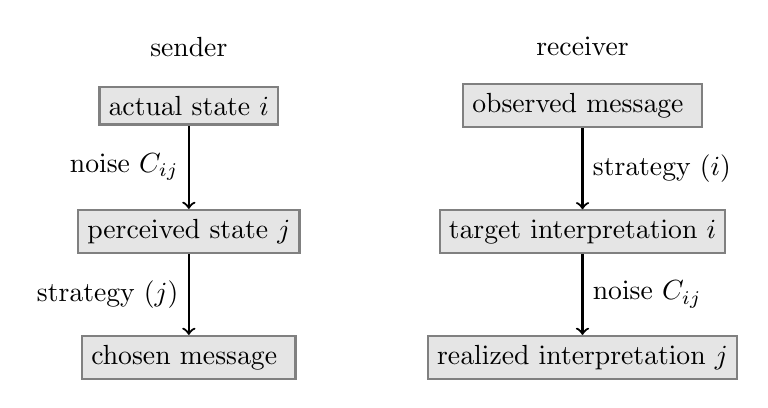
\begin{tikzpicture}[node distance = 1.6cm, thick]

      \begin{scope}
  
      \node[rectangle, draw=black!50, fill=black!10, thick] (actual)
      {actual state $\mystate{i}$};

      \node[rectangle, draw=black!50, fill=black!10, thick, below of =
      actual] (perceived) {perceived state $\mystate{j}$};

      \node[rectangle, draw=black!50, fill=black!10, thick, below of =
      perceived] (output) {chosen message $\messg$};

      \node[rectangle, thick, above of = actual, node distance=0.75cm]
      (sender) {sender};

      \draw[->] (actual) -> (perceived) node[midway,left] {noise
        $C_{ij}$};

      \draw[->] (perceived) -> (output) node[midway,left] (label)
      {strategy $\Sstrat(\messg \probbar \mystate{j})$};

   
%      \begin{pgfonlayer}{background}
%        \node [draw=black!50, fill=black!20,fit=(actual) (label)
%        (output)] {};
%      \end{pgfonlayer}
    \end{scope}


      \begin{scope}[xshift=5cm]
  
      \node[rectangle, draw=black!50, fill=black!10, thick] (message)
      {observed message $\messg$};

      \node[rectangle, draw=black!50, fill=black!10, thick, below of =
      message] (target) {target interpretation $\mystate{i}$};

      \node[rectangle, draw=black!50, fill=black!10, thick, below of =
      target] (realized) {realized interpretation $\mystate{j}$};

      \node[rectangle, thick, above of = message, node distance=0.75cm]
      (receiver) {receiver};

      \draw[->] (message) -> (target) node[midway,right] (bla) {strategy
        $\Rstrat(\mystate{i} \probbar \messg)$};

      \draw[->] (target) -> (realized) node[midway,right]  {noise $C_{ij}$};

   
%      \begin{pgfonlayer}{background}
%        \node [draw=black!50, fill=black!20,fit = (message) 
%        (realized) (bla)] {};
%      \end{pgfonlayer}
    \end{scope}

  \end{tikzpicture}

  \caption{Effect of confusion of states on sender and receiver
    choices.}
  \label{fig:noise-perturbation-of-strategies}
\end{figure}

The aggregate effect of confusion of states on behavioral strategies
can be captured in a function that maps behavioral strategies
$\Sstrat$ and $\Rstrat$ to their \emph{diffusions} $D(\Sstrat)$ and
$D(\Rstrat)$. Suppose that $\Sstrat$ and $\Rstrat$ represent a
population's average signaling behavior if there was no confusion of
states. Then $D(\Sstrat)$ and $D(\Rstrat)$ give the expected aggregate
population behavior under the actual noise-perturbed behavior of each
agent. Since the effect of confusion of states is that behavior at one
choice point percolates to behavior at similar choice points, we speak
of \emph{diffusion of behavior under confusion of states}. If we
conceive of behavioral strategies $\Sstrat$ and $\Rstrat$ as
row-stochastic matrices (rows are choice points, columns are choices;
each row is a probability distribution), the diffusion effect of
confusion matrix $C$ is just matrix multiplication:
\begin{align}
  \label{eq:confusion-function}
  \Diff_C(\Sstrat) & = C \Sstrat &    \Diff_C(\Rstrat) & = \Rstrat C\,.
\end{align}

The discrete-time replicator diffusion dynamic takes the replicator
dynamic as basic, but factors in the confusion of states at each step
in a sequential manner:
\begin{align*}
  \RDD(\Sstrat) & = \Diff_C(\RD(\Sstrat)) &   \RDD(\Rstrat) & = \Diff_C(\RD(\Rstrat)) \,.
\end{align*}
This is equivalent to the following, perhaps more transparent
formulation:\footnote{To see this, start with $\RDD(\Sstrat)(\messg_k
  \probbar \state_i)$. If $\RDD(\Sstrat)$ is considered as a matrix,
  we can rewrite this as $(RDD(\Sstrat)_{ik}$. By
  Equation~(\ref{eq:confusion-function}), we get $(C \
  \RD(\Sstrat))_{ik}$, which by definition of matrix multiplication is
  $\sum_j C_{ij} \cdot \RD(\Sstrat)_{jk}$. Substituting the definition
  of $\RD(\Sstrat)$ completes the derivation. Similarly for the
  receiver.}
\begin{align*}
  \RDD(\Sstrat)(\messg_k \probbar \state_i) & = \sum_{j} C_{ij} \cdot
  \frac{\Sstrat(\messg_k \probbar \state_j) \cdot
    \EU(\messg_k, \state_j,\Rstrat)}
  {\Phi(\state_j,\Sstrat, \Rstrat)} \\
    \RDD(\Rstrat)(\state_i \probbar \messg_k) & = \sum_{j} C_{ji} \cdot
  \frac{\Rstrat(\state_j \probbar \messg_k) \cdot
    \EU(\state_j, \messg_k,\Sstrat)} {\Phi(\messg_k,\Sstrat, \Rstrat)}  \,.
\end{align*}

The most straightforward interpretation of this sequential definition
is that the \rdd captures the most likely path of development of
aggregate behavior in a society, in which behavioral changes occur
independently at each choice point, as described by the \rd for
behavioral strategies. Whatever strategy an agent does actually hold,
its realization is perturbed by imperfect discriminability of states
in such a way that the expected overall aggregate behavior is the
diffusion of the strategies that the agents would play in a noise-free
world. Any agent-level interpretation of the \rd in behavioral
strategies seems \emph{prima facie} compatible with this
interpretation.

The sequential definition highlights that other (discrete-time)
evolutionary dynamics can be subjected to state-confusability in an
analogous fashion. It is easy, for instance, to perturb a
best-response dynamic in case we wanted to model cognizing, rational
agents with a noisy perceptual system. Our choice of the \rd as a
carrier dynamic is motivated by its generality and austerity, being
compatible with a variety of implicit agent-level behavior, without
presupposing extravagant higher cognitive abilities
\citep[c.f.][]{Sandholm2013:Population-Game}. Moreover, by using the
\rd as a carrier for diffusion, we actually obtain a special case of a
behavioral-strategy version of the replicator mutator dynamics. This
is important to know because it enables similar applications of
diffusion from perceptual confusion also in models of biological
evolution.

The following section works out the relation between the \rdd and the \rmd.
Although this section is conceptually important, it is also rather
technical and not strictly necessary to appreciate the main point of
the paper.

%%%%%%%%%%%%%%%%%%%%%%%%%%%%%%%%%%%%%%%%%%%%%%%%%%
%%%%%%%%%%%%%%%%%%%%%%%%%%%%%%%%%%%%%%%%%%%%%%%%%%
\section{Diffusion as mutation}
\label{sec:diffusion-as-special}

\subsection{The replicator mutator dynamic}
\label{sec:repl-mutat-dynam}

The \rmd has first been proposed as a tool for studying the evolution
of grammar
\citep[e.g.][]{KomarovaNiyogi2001:The-Evolutionar,NowakKomarova2001:Evolution-of-Un}. It
adds stochastic mutation to the replicator dynamic. The relation of
the \rmd to other prominent evolutionary dynamics is well understood
\citep{PageNowak2002:Unifying-Evolut}. The \rmd has seen further
fruitful applications in the context of signaling games
\citep[e.g.][]{HutteggerSkyrms2010:Evolutionary-Dy}.

The usual formulation of the \rmd is based on mixed, not behavioral
strategies. But a discrete-time formulation of the \rmd in behavioral
strategies clearly identifies the \rdd to be a special case. It
follows that a mixed strategy version of the \rdd is just the \rmd
with suitably defined mutation matrices. From this, even a
continuous-time version can easily be retrieved if desired. To show
this, we start with a delineation of mixed and behavioral strategies.

\paragraph{Mixed strategies.} Pure sender (receiver) strategies are
functions $\Spure \in \Messgs^\States$ ($\Rpure \in
\Acts^\Messgs$). Mixed sender (receiver) strategies are functions
$\Smixed \in \Delta(\Messgs^\States)$ ($\Rmixed \in
(\Acts^\Messgs)$). The latter give the relative population frequencies
of the former. We write $\Smixed_i$ for the frequency
$\Smixed(\Spure_i)$ of pure strategy $\Spure_i$. Likewise for the
receiver.

Every mixed strategy $\Smixed$ converts to a unique behavioral
strategy defined by:
\begin{align}
  \label{eq:CorrespondenceBehavioralMixed}
  \Sstrat(\messg \probbar \state) = \sum_{\Spure(\state) = \messg} \Smixed(\Spure)\,.
\end{align} 
Let $G$ be this mapping from mixed to behavioral strategies. Note that $G$
is \emph{not} an injection, as many mixed strategies map onto the same
behavioral strategy. In this sense, mixed strategies hold more
information than behavioral strategies about the distribution of pure strategies in a population.

In the context of evolutionary dynamics for signaling games (where
each agent only chooses once), we can think of behavioral strategies
as treating each choice point as an independent update site
\citep[e.g.][]{Cressman2003:Evolutionary-Dy}. Dynamics for mixed
strategies conceive of agents as adjusting their entire pure
strategy. In this way, dependencies between different choices at
different choice points can matter to the evolutionary path. In
contrast, dynamics for behavioral strategies conceive of agents as
adjusting their strategies locally at each choice point, regardless of
what they are disposed to do at other choice points.

This can matter to evolutionary dynamics. For illustration, take two
sender strategies whose behavior is different only at two
states. Compared to the second strategy, the first scores a much
higher expected utility at one state, but a slightly lower at the
other, so that the total expected utility of the first strategy is
higher. Under evolutionary dynamics that work on entire strategies the
first strategy will increase in proportion, relative to the
second. Consequently, a locally less efficient type of behavior can be
promoted because it is correlated with efficient behavior at another
choice point. Evolutionary dynamics working on behavioral strategies
do not allow for that. Behavioral adaptations occur independently at
different choice points.

As a result, dynamics on behavioral strategies are more coarse-grained
and not necessarily equivalent to dynamics on mixed strategies. An
advantage of dynamics in behavioral strategies is that they reduce
complexity, which helps with numerical simulations. They might also be
a more natural choice for cultural dynamics, e.g., when an agent
observes and imitates another agent's strategy: it may be more
plausible that agents adopt the use of a single word, not an entire
lexicon, so to speak. On the other hand, biological evolution seems
more naturally modeled in terms of mixed strategies, since it is a full
set of behavioral disposition that is bequeathed to the next
generation.

\paragraph{Replicator dynamic in mixed strategies.} To understand the
\rmd in mixed strategies, we first introduce the \rd in mixed
strategies. Let $F_i^{\Rmixed}$ be $\Spure_i$'s fitness given
$\Rmixed$ and $F_i^{\Smixed}$ be $\Rpure_i$'s fitness given
$\Smixed$. Then $\Phi(\Smixed,\Rmixed) = \sum_{k} \Smixed_k \cdot
F_k^{\Rmixed}$ is the average fitness in the sender population and
$\Phi(\Rmixed,\Smixed) = \sum_{k} \Rmixed_k \cdot F_k^{\Smixed}$ the
average fitness in the receiver population.

% The continuous-time replicator dynamic defines the change of frequency
% of mixed strategies. Its so-called two-population version, that takes
% sender and receiver roles as separate update sites is:
% \begin{align*}
%   \dot{\Smixed_i} & = \Smixed_i \cdot \left ( F_i^{\Rmixed} -
%   \Phi(\Smixed,\Rmixed) \right ) &   \dot{\Rmixed_i} &  = \Rmixed_i \cdot \left ( F_i^{\Smixed} -
%   \Phi(\Rmixed,\Smixed) \right ) \,.
% \end{align*}
Similar to the version for behavioral strategies, a discrete-time
formulation of the \rd for mixed strategies can be conceptualized as an
update function that maps mixed strategies $\Smixed$ and $\Rmixed$
onto mixed strategies $\RD(\Smixed)$ and $\RD(\Rmixed)$ respectively,
such that:
\begin{align*}
  \RD(\Smixed)_i & = \frac{\Smixed_i \cdot F_i^{\Rmixed}}{
    \Phi(\Smixed,\Rmixed)} & \RD(\Rmixed)_i & = \frac{\Rmixed_i \cdot
    F_i^{\Smixed}}{ \Phi(\Rmixed,\Smixed)} \,.
\end{align*}


\paragraph{Replicator mutator dynamic.} The replicator mutator dynamic
extends the \rd by adding probabilistic mutation. Let $Q$ be a
row-stochastic mutation matrix where $Q_{ji}$ gives the probability
that pure sender strategy $\Spure_j$ mutates into
$\Spure_i$. Similarly, let $R$ be a row-stochastic mutation matrix
where $R_{ji}$ gives the probability that pure receiver strategy
$\Rpure_j$ mutates into $\Rpure_i$.

The \rmd is usually given only in its continuous-time form. % A
% two-population (non-payoff adjusted) formulation is then:
% \begin{align*}
%   \dot{\Smixed_i} & = \sum_{j}  Q_{ji} \cdot \Smixed_j
%     \cdot F_j^{\Rmixed} - \Smixed_i \cdot \Phi(\Smixed,\Rmixed) &
%     \dot{\Rmixed_i} & = \sum_{j}  R_{ji} \cdot \Rmixed_j
%     \cdot F_j^{\Smixed} - \Rmixed_i \cdot \Phi(\Rmixed,\Smixed) \,.
% \end{align*}
But a discrete-time, two-population formulation of the \rmd is
available too \citep[c.f.][97]{PageNowak2002:Unifying-Evolut}:
\begin{align*}
  \RMD(\Smixed)_i & = \sum_{j} Q_{ji} \frac{\Smixed_j \cdot
    F_j^{\Rmixed}}{ \Phi(\Smixed,\Rmixed)} & \RDD(\Rmixed)_i & =
  \sum_{j} R_{ji} \frac{\Rmixed_j \cdot F_j^{\Smixed}}{
    \Phi(\Rmixed,\Smixed)}\,.
\end{align*}
The discrete-time \rmd has the same sequential nature as the \rdd:
first we compute the fitness-driven change according to the standard
replicator dynamic; then we compute the perturbation from
mutation. This becomes clear if we define independent mutation
functions $\Mutate_{Q,R}$ that map mixed strategies onto the outcome
of (one round of) mutation:
\begin{align}
  \label{eq:Mutation}
  \Mutate_Q(\Smixed)_i & =  \sum_j  \Smixed_j \cdot
  Q_{ji} &   \Mutate_R(\Rmixed)_i & =  \sum_{j}  \Rmixed_j \cdot
  R_{ji} \,.
\end{align}
The discrete-time \rmd given above can then be rewritten as:
\begin{align*}
  \RDD(\Smixed) &= \Mutate_Q(\RD(\Smixed)) &   \RDD(\Rmixed) &= \Mutate_R(\RD(\Rmixed))\,. 
\end{align*}

\subsection{Relating the dynamics}

The sequential reformulation of the \rmd closely resembles our initial
formulation of the \rdd. However, there is a major difference between
these. While the \rdd is a dynamic for behavioral strategies, the
\rmd, as taken from the literature, applies to mixed
strategies. Similarly, the confusability of states is an operation
that is straightforwardly definable for behavioral strategies (see
Equation~(\ref{eq:confusion-function})), while mutation in the \rmd is
defined as mutation from one pure strategy to another. Nonetheless, it
is possible to map each confusion matrix to a mutation matrix in a
natural way so that the correspondence between mixed and behavioral
strategies are conserved. This is the main result presented in this
section, and it is our justification for regarding the \rdd as the
behavioral-strategy analogue of the replicator-mutator dynamic when
the only source of mutation is confusability of states.

\begin{figure}
  \centering
  
  \begin{tikzpicture}[node distance = 1cm]
    
    \begin{scope}
      \node[] (mixed) {$\Smixed$};

      \node[below of = mixed] (mutated) {$\Mutate_{Q^C}(\Smixed)$};

      \node[left of = mixed, node distance = 1.5cm] (dummyl) {};

      \node[right of = mixed, node distance = 1.5cm] (dummyr) {};

      \draw[->, dotted, thick] (mixed) -> (mutated);

  
      \begin{pgfonlayer}{background}
        \node [draw=black!50, fill=black!10,fit = (dummyl) 
        (mutated) (dummyr)] (mixedSpace) {};
      \end{pgfonlayer}

      \node[above of = mixedSpace, node distance = 1.4cm] {space of
        mixed strategies};
    \end{scope}

    \begin{scope}[xshift=6cm]
      \node[] (behavioral) {$\Sstrat$};

      \node[below of = behavioral] (mutatedBeh) {$\Diff_C(\Sstrat)$};

      \node[left of = behavioral, node distance = 1.5cm] (dummylB) {};

      \node[right of = behavioral, node distance = 1.5cm] (dummyrB) {};

      \draw[->, dotted, thick] (behavioral) -> (mutatedBeh);

  
      \begin{pgfonlayer}{background}
        \node [draw=black!50, fill=black!10,
              fit = (dummylB) (mutatedBeh) (dummyrB)] (behSpace) {};
      \end{pgfonlayer}

      \node[above of = behSpace, node distance = 1.4cm] {space of
        behavioral strategies};
    \end{scope}

    \draw[->,thick,dotted] (mixed) -> (behavioral) node[midway,
    above]{$G(\Smixed)$};

    \draw[->,thick,dotted] (mutated) -> (mutatedBeh) node[midway, below]{$G(\Mutate_{Q^C}(\Smixed))$};

  \end{tikzpicture}

  \caption{Correspondence between state-confusion and mutation.}
  \label{fig:correspondence-result}
\end{figure}

More concretely, given the non-injective mapping $G$ from mixed to
behavioral strategies, we show that there is a systematic translation
from a confusion matrix $C$ to a mutation matrix $Q^C$ such that for
each mixed sender strategy $\Smixed$, its unique corresponding
behavioral strategy $\Sstrat = G(\Smixed)$ has a
confusion-perturbation $\Diff_C(\Sstrat)$ that corresponds, via $G$,
to the mutation-perturbation $\Mutate_{Q^C}(\Smixed)$ (see
Figure~\ref{fig:correspondence-result}). In other words, we
hypothesize that a confusion matrix $C$ should give rise to a unique
mutation matrix $Q^C$ so that whenever $G(\Smixed) = \Sstrat$ we also
have $G(\Mutate_{Q^C}(\Smixed)) = \Diff_C(\Sstrat)$. Similarly, for
the receiver.
%This is the content of Theorem~\ref{thm:Correspondence} given below, a
%proof for which is in Appendix~\ref{sec:proofs}. The remainder of this
%section introduces the relevant construction that maps arbitrary $C$
%to suitable $Q^C$.

\paragraph{Confusion-based mutations.} There are natural conversions
of $C$ into $Q^C$ and $R^C$. The case for the receiver is easier, so
we start with that.

The probability that $\Rpure_i$ is realized as $\Rpure_j$ under
diffusion with $C$ is the product of the probabilities, for each
$\messg$, that the state $\Rpure_i(\messg)$ is perceived as state
$\Rpure_j(\messg)$. Abusing notation by referring to the indices of
states $\Rpure_i(\messg)$ and $\Rpure_j(\messg)$ with
$\Rpure_i(\messg)$ and $\Rpure_j(\messg)$ directly, we define:
\begin{align}
  \label{eq:construction-rec}
  R^C_{ij} = \prod_{\messg} C_{\Rpure_i(\messg)\Rpure_j(\messg)}\,.
\end{align}

Now look at the sender. The probability that $\Spure_j$ is realized as
$\Spure_i$ under diffusion with $C$ is the product of the
probabilities, over all states $\mystate{k}$, that the message
$\Spure_i(\mystate{k})$, that $\Spure_i$ would produce at state
$\mystate{k}$ in the absence of noise, is produced by a noisy
realization of $\Spure_j$, which is the probability $\sum_{\state_l
  \in \Spure_j^{-1}(\Spure_i(\state_k))} C_{kl}$ that the state
$\mystate{k}$ is realized as a state $\mystate{l}$ which $\Spure_j$
would map unto $\Spure_i(\mystate{k})$. So, define:
\begin{align}
  \label{eq:construction-sen}
  Q^C_{ji} = \prod_{\state_k} \sum_{\state_l \in
    \Spure_j^{-1}(\Spure_i(\state_k))} C_{kl}\,.
\end{align}

Based on Equations~(\ref{eq:construction-rec}) and
(\ref{eq:construction-sen}), we can formulate the desired
correspondence result, a proof for which is given in Appendix~\ref{sec:proofs}.

\begin{theorem}
  \label{thm:Correspondence}
  (i) If $G(\Smixed) = \Sstrat$, then $G(\Mutate_{Q^C}(\Smixed)) =
  \Diff_C(\Sstrat)$. (ii) If $G(\Rmixed) = \Rstrat$, then
  $G(\Mutate_{R^C}(\Rmixed)) = \Diff_C(\Rstrat)$.
\end{theorem}


%%%%%%%%%%%%%%%%%%%%%%%%%%%%%%%%%%%%%%%%%%%%%%%%%%
%%%%%%%%%%%%%%%%%%%%%%%%%%%%%%%%%%%%%%%%%%%%%%%%%%

\section{Exploring the RDD}
\label{sec:exploring-rdd}

The previous sections showed that the \rdd can be conceptualized as a
two-step procedure: we first calculate where the replicator dynamic
would take us, then apply diffusion. To understand the \rdd better, we
isolate the novel diffusion part in
Section~\ref{sec:iterated-diffusion}, before exploring how diffusion
and fitness-based selection interact in Section~\ref{sec:simulations}.

\subsection{Iterated diffusion}
\label{sec:iterated-diffusion}

Confusion of states should intuitively be a function of their
perceptual similarity. To make this concrete, let us assume that the
state space of the sim-max game consists of $n \ge 2$ states that are
equally spaced across the unit interval, including $0$ and $1$. The
distance $\card{\mystate{i} - \mystate{j}}$ is the objective, physical
similarity between two states $\mystate{i}$ and
$\mystate{j}$. Distance in physical space feeds into a perceptual
similarity function, as described by
\citet{Nosofsky1986:Attention-Simil}:
\begin{align*}
  \similarity(\mystate{i}, \mystate{j} \myts ; \myts \impairment) =
      \begin{cases}
    1 & \textrm{if } \impairment = 0 \textrm{ and } \mystate{i} = \mystate{j} \\
    0 & \textrm{if } \impairment = 0 \textrm{ and } \mystate{i} \neq \mystate{j} \\
 \expo \left ( -  \frac{\card{\mystate{i} - \mystate{j}}^s}{ \impairment^2} \right ) & \textrm{otherwise,} \\
    \end{cases}
\end{align*}
where $\impairment \ge 0$ is an imprecision or indiscriminability
parameter. When $\impairment=0$ agents perfectly discriminate between
states; when $\impairment \rightarrow \infty$ agents cannot
discriminate states at all. Figure~\ref{fig:NosofskySim} gives an
impression of Nosofsky-similarity for different parameter
values. Other formalizations of perceptual similarity are possible,
including ones that allow for different discriminability in different
areas of the state space, but we stick with Nosofsky's similarity
function for the time being, because it is mathematically simple, yet
an established notion in mathematical psychology.

\begin{figure}
  \centering

  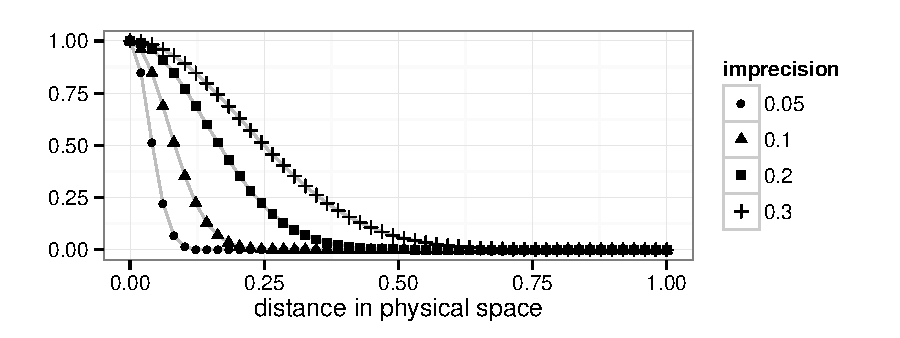
\includegraphics[width=0.7\textwidth]{plots/NosofskySim.pdf}

  \caption{Examples of Nosofsky-similarity for different values of
    imprecision.}
  \label{fig:NosofskySim}
\end{figure}


We further assume that the probability of confusing any two states
$\mystate{i}$ and $\mystate{j}$ is proportional to their perceived
similarity and therefore obtained by normalization:
\begin{align*}
  C_{ij} = \frac{\similarity(\mystate{i}, \mystate{j} \myts ; \myts
  \impairment)} {\sum_j \similarity(\mystate{i}, \mystate{j} \myts ; \myts
  \impairment)} \,.
\end{align*}
Confusion of states is then also a function of imprecision parameter
$\impairment$. For $\impairment = 0$, the confusion matrix has $C_{ii}
= 1$; for $\impairment > 0$, $C$ is positive, i.e., $C_{ij} >0$ for
all $i$ and $j$; for $\impairment \rightarrow \infty$, we find $C_{ij}
= \nicefrac{1}{\card{\States}}$ for all $i$ and $j$.

If states are confused on average with a probability proportional to
their similarity, repeated application of the operation in
Equation~(\ref{eq:confusion-function}) causes behavioral dispositions
gradually to diffuse along a gradient of similarity of
states. Consequently, iterated diffusion leads to a smoothing out and
an eventual equalization of behavioral strategies, for both the sender
and the receiver. After $n$ steps of iterated diffusion an initial
sender strategy $\Sstrat$ will be $C^n \Sstrat$, and an initial
receiver strategy $\Rstrat$ will be $\Rstrat C^n$. If we assume that
$\impairment > 0$, $C$ is a positive row-stochastic matrix (each state
could in principle be confused as any other state, albeit with
possibly a very low probability). It then follows from the
Perron-Frobenius theorem that the limit $C^\infty = \lim_{n
  \rightarrow \infty} C^n$ exists (it is the Perron-projection) and
all of its rows are identical. That is why, in the limit of iterated
diffusion, $C^\infty \Sstrat$ has identical rows (messages are sent
with the same probability in each state), and $\Rstrat C^\infty$
likewise has identical rows (every message is interpreted
equally). All of this is in line with the intuition that diffusion of
behavior under confusion of states iteratively equalizes behavior for
similar states; if all states can be confused for one another in
principle, behavior smoothes out entirely in the limit.

\subsection{Numerical simulations}
\label{sec:simulations}

Now that we understand better what diffusion does, let us look at how
diffusion interacts with optimization of behavior, as described by the
replicator dynamics. The main question we should address is whether
diffusion and fitness-based replication reasonably interact, and if
so, whether the inclusion of diffusion has any noteworthy effects on
the evolving meaning of signals. Clearly, if $\impairment = 0$, the
\rdd reduces to the \rd. If $\impairment \rightarrow \infty$, the
diffusion component takes over and the \rdd reduces to the trivial
iterated diffusion process that we looked at in the previous
section. We will show presently that for reasonable in-between levels
of imprecision $\impairment$, the \rdd can lead to reasonably
efficient, yet vague signaling behavior. Suitable levels of
imprecision can have further accelerating and, surprisingly, unifying
effects on meaning evolution.

\subsubsection{Experimental set-up}

To explore the \rdd, we turn to numerical simulations. Let states be
evenly spaced elements of the unit interval that always include 0 and
1, and let priors be flat: $\Pr(\state) = \Pr(\state')$ for all
$\state, \state'$. As for utility functions, we take another
Nosofsky-style function:
\begin{align*}
  \util(\mystate{i}, \mystate{j} \myts ; \myts \toler) =
      \begin{cases}
    1 & \textrm{if } \toler = 0 \textrm{ and } \mystate{i} = \mystate{j} \\
    0 & \textrm{if } \toler = 0 \textrm{ and } \mystate{i} \neq \mystate{j} \\
 \expo \left ( -  \frac{\card{\mystate{i} - \mystate{j}}^s}{ \toler^2} \right ) & \textrm{otherwise.} \\
    \end{cases}
\end{align*}
The tolerance parameter $\toler \ge 0$ models the amount of tolerable
pragmatic slack or communicative imprecision. This choice of utility
function is governed partly by convenience in parallel to the
similarity function, but also because it has, as we believe, the right
general properties for a communicative payoff function. Unlike
utilities that are, say, linearly or quadratically decreasing in
physical distance \citep[c.f.][]{JagerMetzger2011:Voronoi-Languag,FrankeJager2010:Vagueness-Signa},
utilities that are exponentially decreasing in negative quadratic
distance can model situations where a small amount of imprecision in
communication is tolerable, whereas similarly small differences in
intolerably far away interpretations matter very little, with a smooth
transition between these regimes
\citep[c.f.][]{OConnor2013:The-Evolution-o}.

\begin{figure}
  \centering

  \begin{subfigure}[]{0.45\textwidth}
    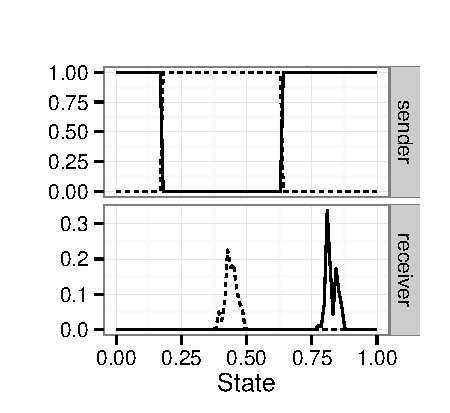
\includegraphics[width=\textwidth]{plots/strat_example_ind3098.pdf}
    \caption{$\ns = 90$, $\toler = 0.1$, $\impairment = 0$}
    \label{fig:example_stratsA}
  \end{subfigure}
  \hfill
  \begin{subfigure}[]{0.45\textwidth}
    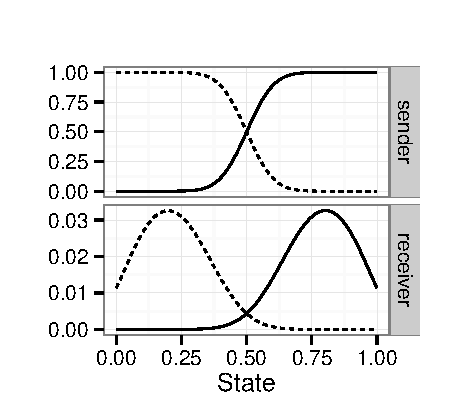
\includegraphics[width=\textwidth]{plots/strat_example_ind3452.pdf}
    \caption{$\ns = 90$, $\toler = 0.1$, $\impairment = 0.1$}
    \label{fig:example_stratsB}
  \end{subfigure}

  % \begin{subfigure}[]{0.45\textwidth}
  %   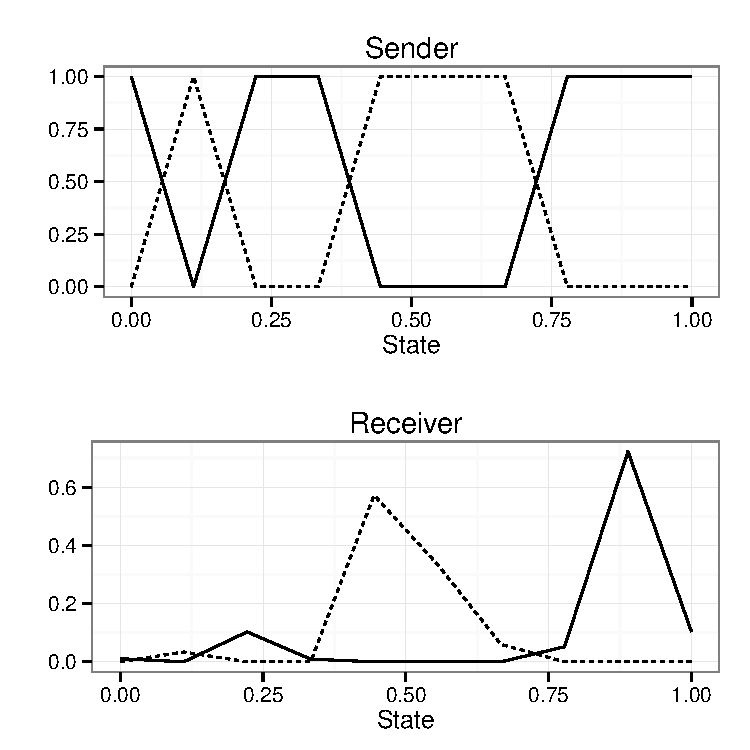
\includegraphics[width=\textwidth]{plots/strat_example_NS-10_tol-005_imp0_ind1001.pdf}
  %   \caption{$\ns = 10$, $\toler = 0.1$, $\impairment = 0$}
  %   \label{fig:example_stratsC}
  % \end{subfigure}
  % \hfill
  % \begin{subfigure}[]{0.45\textwidth}
  %   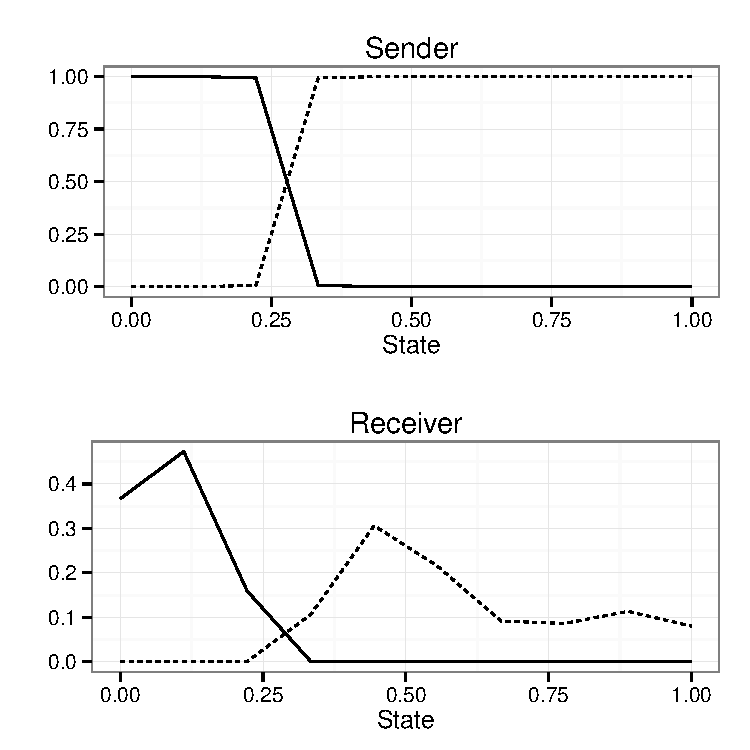
\includegraphics[width=\textwidth]{plots/strat_example_NS-10_tol-005_imp005_ind1201.pdf}
  %   \caption{$\ns = 10$, $\toler = 0.1$, $\impairment = 0.05$}
  %   \label{fig:example_stratsD}
  % \end{subfigure}


  \caption{Example strategies under \rdd at stopping time of our simulations.}
  \label{fig:example_strats}
\end{figure}

We ran 50 trials of the \rdd, starting with randomly sampled sender
and receiver strategies, for each triplet of independent parameter
values: $\ns = \card{T} \in \set{6, 10, 50, 90}$, $\impairment \in
\set{0, 0.05, 0.1, 0.2, 0.3}$, $\toler \in \set{0.05, 0.1, 0.2,
  0.3}$. Each trial ran for a maximum of 200 update steps of the
\rdd. A trial was considered converged, and thus stopped before the maximum
of 200 rounds, if the total amount of change between strategies before
and after an \rdd step was smaller than a suitably chosen
threshold. It is not guaranteed that strategies at halting time had
converged to the eventual attracting state, whether they ran for 200
rounds or not. Our notion of convergence is therefore only a
categorical measure for reaching a certain (well-considered, but
eventually arbitrary) degree of stability. In principle, rather than
setting a hard limit on the maximum number of rounds and analyzing
convergence categorically, one could also run each trial until reaching
our criterion for convergence and analyze the number of rounds it took to get there.
Our choice was initially motivated by pragmatic concerns regarding length of
simulation time, but it is also justifiable if we reflect on the
nature of language evolution as a continuous process.
Language adapts to an ever-changing reality; it is rare, if not impossible,
that a lexicon has an infinite amount of time to neatly converge to a stable
state. Therefore, investigating speed of convergence within a limited
time frame can be seen as better reflecting the natural constraints of
language evolution.

Representative examples for resulting strategy pairs are given in
Figure~\ref{fig:example_strats}. Figure~\ref{fig:example_stratsA}
shows a strategy pair at stopping time with 90 states, tolerance
$\toler = 0.1$ and imprecision $\impairment = 0$. Zero imprecision
means that the trial was effectively an application of the plain
\rd. Noteworthily, the given sender strategy approximates a pure
sender strategy that crisply partitions the state space into
non-convex sets. The irregular shape of the receiver strategy shows
clearly that the pictured strategy pair has not yet reached a
dynamically stable state under the \rd. Indeed, the trial was stopped
after the maximum of 200 rounds. In contrast, the outcome of a trial
with identical parameters, except with imprecision $\impairment =
0.1$, which is shown in Figure~\ref{fig:example_stratsB}, had
converged (in our technical sense) after 99 rounds of iterated
\rdd. The sender strategy shows a smooth blending from one
``category'' to the other, and the receiver's interpretations are
rather extended curves, peaking at a central point in the relevant
``categories.''

These examples already show two interesting things. Firstly, inclusion
of imprecision can lead to seemingly well-behaved, yet vague
strategies in the sense that we are after. The sender strategy in
Figure~\ref{fig:example_stratsB} identifies clear positive and clear
negative cases for each signal, with a smooth transition
in-between. The receiver's interpretations of signals can be seen as
smoothed-out prototype regions. Secondly, (sender) strategies can
approach non-convex pure strategies under the replicator dynamic and
linger there for vast amounts of time, possibly indefinitely. We see
this in our limited-time simulations, but this also holds, for some
types of utility functions, for the limiting case. This was first
observed by Elliott Wagner in unpublished work
\citep[c.f.][]{OConnor2013:Evolving-Percep}. A full analysis of the
dynamics of sim-max games is beyond the scope of this paper, but we
will see shortly that diffusion from confusability of states clearly
prevents evolutionary paths that meander for a long time in the
vicinity of non-convex strategies.



\subsubsection{Dependent measures}
 
To further explore our simulation results, we calculated metrics that
aim to numerically capture how vague, generally well-structured, and
communicatively efficient the recorded strategy pairs
were. \emph{Entropy} captures the amount of systematicity or
regularity in signal use. \emph{Convexity} captures whether a
behavioral strategy would project onto a convex pure
strategy. \emph{Expected utility} measures the communicative
efficiency of evolved strategy pairs.

\paragraph{Entropy.} This classic information-theoretic notion
captures the amount of uncertainty in a probability
distribution. Roughly put, entropy of a signaling strategy captures
inverse distance from a pure strategy. The usual definition of entropy
applies directly to mixed strategies, but provably equivalent metrics
for behavioral strategies are ready to hand:
\begin{align*}
  E(\Sstrat) = -\sum_{\state \in \States} \sum_{\messg \in \Messgs}
  \Sstrat(\messg \probbar \state) \cdot \log(\Sstrat(\messg \probbar
  \state)) \\
  E(\Rstrat) = -\sum_{\messg \in \Messgs} \sum_{\state \in \States}
  \Rstrat(\state \probbar \messg) \cdot \log(\Rstrat(\state \probbar
  \messg)) \,. 
\end{align*}
Values obtained by these definitions are lower bounded by $0$ and
upper bounded by, respectively, $\log(|\Messgs^\States|) = |\States|
\cdot \log(|\Messgs|)$ and $\log(|\States^\Messgs|) = |\Messgs| \cdot
\log(|\States|)$. We work with normalized values. The sender
strategies in Figures~\ref{fig:example_stratsA} and
\ref{fig:example_stratsB} have entropy $1.19e^{-5}$ and $0.21$,
respectively. The receiver strategies have respective entropies $0.43$
and $0.84$. In general, we expected that vague languages would have
higher entropy than crisp ones and that increasing imprecision would
lead to increased entropy, all else being equal.

\paragraph{Convexity.} At least for sender strategies, which develop
faster than receiver strategies, it also makes sense to define a
categorical measure of convexity that compensates for potential
vagueness. To determine whether a sender strategy $\Sstrat$ is convex
despite possibly being vague, we look at the derived pure strategy
$\Spure$ for which $\Spure(\state) = \argmax_{\messg' \in \Messgs}
\Sstrat(\state,\messg')$. If that $\Spure$ is convex, we also count
$\Sstrat$ as convex. The sender strategy in
Figure~\ref{fig:example_stratsA} is not convex, while the one in
Figure~\ref{fig:example_stratsB} is.  One would a priori not expect a
systematic relation between imprecision and convexity.

\paragraph{Expected utility.} We also recorded the expected utility of
a strategy pair:
\begin{align*}
  \EU(\Sstrat,\Rstrat \myts ; \myts \toler) = \sum_{\state \in
    \States} \sum_{\messg \in \Messgs} \sum_{\state' \in \States}
  \Pr(\state) \cdot \Sstrat(\state, \messg) \cdot \Rstrat(\messg,
  \state') \cdot \Util(\state,\state' \myts ; \myts \toler)\,.
\end{align*}
To make direct comparisons across different parameter settings, we
normalize expected utility by the maximal amount of expected utility
obtainable in the relevant game. The strategy pair in
Figure~\ref{fig:example_stratsA} has a normalized expected utility of
$0.992$, the pair in Figure~\ref{fig:example_stratsB} has
$0.901$. Generally, vagueness and imprecision can be expected to
decrease expected utility
\citep[c.f.][]{Lipman2009:Why-is-Language}. The crucial question is
whether communicative success drops unacceptably fast with moderate
levels of vagueness and imprecision.

\subsubsection{Results}

\begin{figure}[t]
  \centering
  
  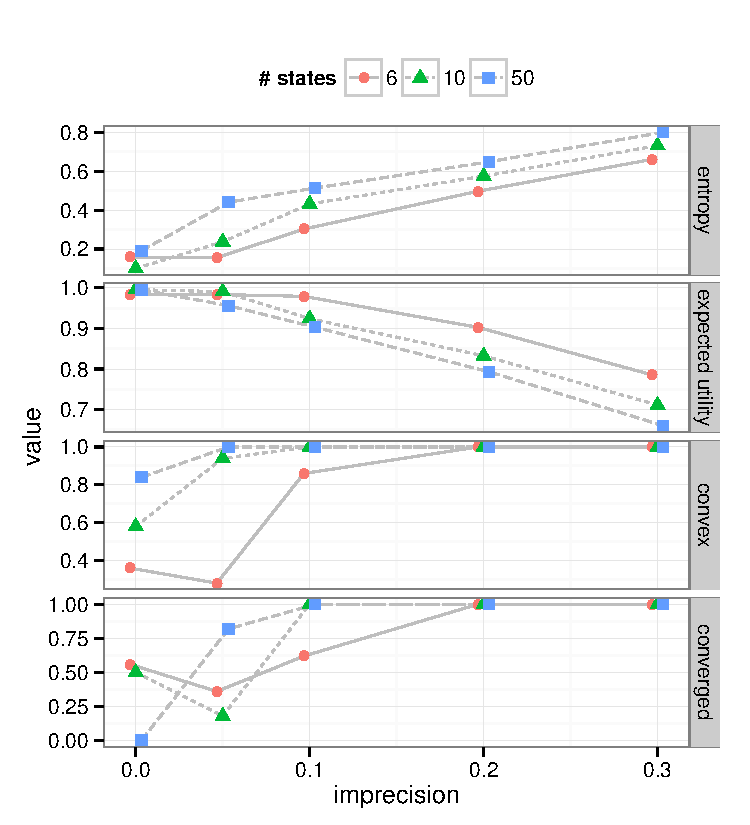
\includegraphics[width=0.75\textwidth]{plots/MeanMetrics3.pdf}

  \caption{Means of gradient and proportions of categorical measures
    for $\toler = 0.1$, $\ns \in \set{6, 10, 50}$, and $\impairment
    \in \set{0, 0.05, 0.1, 0.2, 0.3}$. The plot shows the average of
    the entropies for the sender and receiver strategy.}
  \label{fig:MeanMetrics}
\end{figure}

Figure~\ref{fig:MeanMetrics} shows plots summarizing the results of
our simulation. For perspicuity, we only plot results for one level of
tolerance $\beta = 0.1$, and leave out the case of $n_s = 90$. Still,
every qualitative trend we mention in the following applies to the
whole set of results.

As expected, increasing imprecision leads to higher entropy and lower
expected utility. Importantly, however, imprecision does not
necessarily lead to disastrous decline of communicative success. What
was not expected, on the other hand, was a relation between
imprecision and convexity. However, the corresponding plot clearly
shows that higher imprecision led to a higher number of outcomes with
convex sender strategies. Moreover, it also led to higher likelihood
of convergence. In fact, sufficient impairment always ensured
convergence and convexity. It appears that perceptual imprecision
leads to more vagueness, slightly less communicative efficiency, but
more regular, well-behaved languages in shorter time.

Beyond promoting convexity and convergence, diffusion also has another interesting
regularizing effect on the evolution of signaling. There was very
little variation in the recorded metrics for evolved strategies, at
least for higher values of impairment. On closer inspection, it turns
out that variability in low-impairment conditions is not only due to
non-convergence or non-convexity. Figure~\ref{fig:MoreExample_strats}
gives two more examples of strategy pairs at stopping time. Both are
obtained for the same triple of parameters, both converged before the
maximum number of rounds, and both have
convex sender strategies. However, they are not equally efficient. In
fact, the pair in Figure~\ref{fig:example_stratsC} has a normalized
expected utility of $0.99$ while the one in
Figure~\ref{fig:example_stratsD} only has $0.89$.


\begin{figure}
  \centering

  \begin{subfigure}[]{0.45\textwidth}
    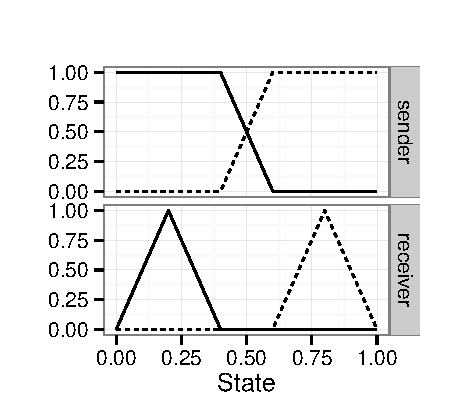
\includegraphics[width=\textwidth]{plots/strat_example_ind21.pdf}
    \caption{$\ns = 6$, $\toler = 0.2$, $\impairment = 0$}
    \label{fig:example_stratsC}
  \end{subfigure}
  \hfill
  \begin{subfigure}[]{0.45\textwidth}
    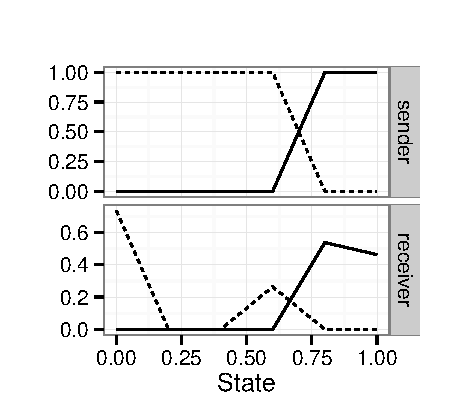
\includegraphics[width=\textwidth]{plots/strat_example_ind23.pdf}
    \caption{$\ns = 6$, $\toler = 0.2$, $\impairment = 0$}
    \label{fig:example_stratsD}
  \end{subfigure}

  \caption{More example strategies under \rdd at stopping time of our simulations.}
  \label{fig:MoreExample_strats}
\end{figure}

Interestingly, this type of variability in evolutionary outcomes can
be weeded out by impairment. To investigate this, we calculated the average
distance between evolved sender strategies within each group of trials
that had identical parameter values. We determined the distance
between strategies $\Sstrat$ and $\Sstrat'$ as the average Hellinger
distance between distributions $\Sstrat(\state)$ and
$\Sstrat'(\state)$ at each choice point $\state$:
\begin{align*}
  \text{HD}(\Sstrat,\Sstrat') & = \frac{1}{{\card{\States} \cdot
     \sqrt{2}}} \cdot  \sum_{\state \in \States} 
 \sqrt{\sum_{\messg \in  \Messgs}
         \left ( \sqrt{\Sstrat(\state,\messg)} -
         \sqrt{\Sstrat'(\state,\messg)} \right )^2 }\,.
\end{align*}
To compensate for the arbitrariness of message use, we set the
distance between strategies $\Sstrat$ and $\Sstrat'$ to be the maximum
of $\text{HD}(\Sstrat,\Sstrat')$ and $\text{HD}(\Sstrat^*,\Sstrat')$
where $\Sstrat^*$ is $\Sstrat$ with reversed message indices. An example of the
\emph{within group distance}, i.e., the average distances between all
sender strategies obtained for the same parameter values, is plotted
on the left in Figure~\ref{fig:GroupMeasures} for $\beta =
0.1$ and $n_s = 10$. Despite some quantitative differences, the
general trend is the same for all other parameter settings that we tested:
with increasing imprecision, the sender strategies evolving under \rdd
were much more alike (modulo swapping of messages). This means that
perceptual imprecision unifies evolutionary outcomes and guarantees
sender strategies that are not only convex, but also regular in that
they induce a vague category split exactly in the middle of the unit
interval.

\begin{figure}
  \centering

    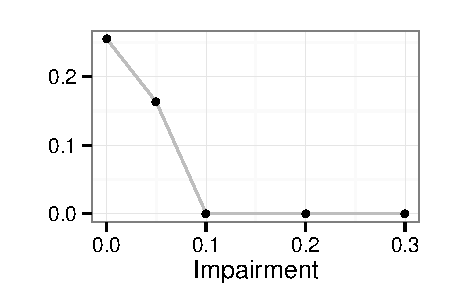
\includegraphics[width=0.475\textwidth]{plots/WithinGroupDistanceConcise.pdf}
    \hfill
    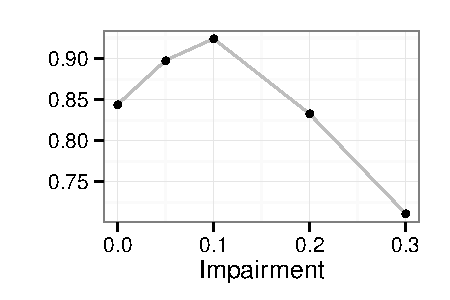
\includegraphics[width=0.475\textwidth]{plots/WithinGroupEUConcise.pdf}

    \caption{Within group distance (left) and within group expected
      utility (right) as a function of impairment for all runs with
      $\toler = 0.1$ and $n_s = 10$.}
  \label{fig:GroupMeasures}
\end{figure}

This unifying property of perceptual imprecision could be considered
an evolutionary beneficial side-effect. Higher imprecision can lead to
higher \emph{within group expected utility}, defined as the average
expected utility that each evolved language (i.e., pair of sender and
receiver strategy at stopping time) scored when playing against an
arbitrary other language obtained for the same parameter values. The
right side of Figure~\ref{fig:GroupMeasures} gives a representative
example. The observation repeats for other parameter values: while
imprecision might decrease the communicative efficiency of individual
languages, it increases the conceptual coherence and communicative
success between independently evolving strategies. It is almost as if
mere confusability of states imposes a regularity constraint on
evolving categories.

%%%%%%%%%%%%%%%%%%%%%%%%%%%%%%%%%%%%%%%%%%%%%%%%%%
%%%%%%%%%%%%%%%%%%%%%%%%%%%%%%%%%%%%%%%%%%%%%%%%%%

\section{Discussion}
\label{sec:discussion}

\subsection{Interpretation of model and results}
\label{sec:model-interpretation}

The \rdd adds expected confusion of similar states to the \rd in
behavioral strategies. The result is an abstract evolutionary dynamic
that describes the most likely path of development of aggregate
population behavior in which any process of behavioral adaptation at
the agent level that is consistent with the \rd in behavioral
strategies is perturbed by systematic noise in the realization of the
agents' strategies. Given the use of behavioral strategies, an
interpretation as a process of cultural evolution is most salient,
according to which agents adapt their choice dispositions locally at
each choice point. But the \rdd is also extensible to biological
evolution on mixed strategies, in which case it is a special case of
the \rmd with mutation matrices derived from confusion matrices, as
shown in Section~\ref{sec:diffusion-as-special}. 

The \rdd is not only compatible with several interpretations of how,
at an agent level, the population-level changes in strategy
proportions come about. It is also compatible with several
interpretations of diffusion. Diffusion can be pictured as a flaw or a
virtue. If we think of perceptual imprecision as a hard limitation on
information processing, vagueness is a natural byproduct of language
evolution. Results from numerical simulations show that such
imprecision leads to vagueness, but does not need to undermine the
prospect of evolving regular and by-and-large efficient signaling
behavior. On the other hand, there appears to be a possibly beneficial
side-effect of state confusability: it speeds up convergence to
regularly shaped and convex categories. This suggests that diffusion
of behavior, as we implemented here, could also be seen as a form
of stimulus-generalization that is evolutionarily beneficial, because
it accelerates the emergence of uniform category formation. This
latter view is also suggested by a like-minded account to which we
turn next.

\subsection{Relation with previous accounts}
\label{sec:relat-with-prev}

\paragraph{Generalized reinforcement.}
% Repeated below...
%\citet{OConnor2013:The-Evolution-o} introduced a generalization of
%Herrnstein reinforcement learning for sim-max games and showed that
%this not only leads to vague signaling patterns, but can speed-up
%evolution of efficient signaling strategies, especially in games with
%many states. 

Under \emph{Herrnstein reinforcement learning}, sender and receiver
adjust their dispositions to act after each round of play, in such a
way that the actual (non-negative) payoff gained in the previous
interaction is added to the non-normalized propensities for repeating
the same behavior. For sim-max games, this means that, when the sender
chose $\messg$ in state $\state$, and this resulted in some
non-negative payoff, the probability that the sender chooses $\messg$
again in $\state$ is increased, but nothing else changes. In
particular, the sender's behavior in other choice points does not
change. \emph{Generalized reinforcement learning} is different. When
the use of $\messg$ in $\state$ gave positive payoff, then not only
will its future use probability be promoted at $\state$ but also at
other states, proportional to how similar these are to
$\state$. Similar amendments take care of the way that the receiver
updates his choice dispositions.

\citet{OConnor2013:The-Evolution-o} shows that this extension not only
leads to vague signaling of the appropriate kind, but also speeds up
learning in such a way that, especially for sim-max games with higher
numbers of states, higher levels of communicative success are reached
in shorter learning periods. Technically, this result is partly due to
the fact that signalers make bigger changes to their behavioral
strategies after each round of play under generalized reinforcement
than under the Herrnstein variety. But that only explains the speed of
adaptation, not necessarily that generalization also leads to
regularity and communicative efficiency, but it does.

Diffusion of strategies in the \rdd can also be conceived of as a form
of generalization, and works in large part quite analogous to stimulus
generalization in \citeauthor{OConnor2013:The-Evolution-o}'s
approach. But there are still
differences. \citeauthor{OConnor2013:The-Evolution-o} showed that
generalized reinforcement learning can speed up the development of
efficient signaling, especially for higher numbers of
states. Complementing this, we showed that diffusion regularizes
evolutionary outcomes and prevents meandering around sub-optimal and
non-convex strategies, also for low numbers of states.

Conceptually, the \rdd is a more abstract framework than generalized
reinforcement learning. The latter is most naturally seen as an
agent-based learning dynamic that has two players adapt their
individual strategies after each concrete round of play. In contrast,
the \rdd describes a more abstract, average dynamical change in
behavioral dispositions at the aggregate population level. Although
the behavior of (some forms of) reinforcement learning mirror those of
the \rd (at some stage in time)
(\cite{BorgersSarin997:Learning-Throug,HopkinsPosch2005:Attainability-o,Beggs2005:On-the-Converge}),
this does not mean that \emph{generalized} reinforcement learning is
also necessarily a plausible population-level description of, say,
generalized learning in a population of agents. Seen in this light,
generalized reinforcement learning and the \rdd nicely complement each
other, as similarly-minded accounts operating at different levels of
abstraction.

\paragraph{Quantal response equilibria.}
\citet{FrankeJager2010:Vagueness-Signa} suggested a number of ways in
which information-processing limitations could lead to vague
strategies. The model that is most clearly related to the present
approach uses the notion of a \emph{quantal response}, also known as a
\emph{soft-max function}
\citep[e.g.][]{Luce1959:Individual-Choi,McFadden1976:Quantal-Choice-,GoereeHolt2008:Quantal-Respons}. A
quantal response function is a parameterized generalization of the
classic best response function. For example, if $U \mycolon \Acts
\rightarrow \mathds{R}$ is the measure of expected utility over
choices $\Acts$ of an agent, then a best response function would have
the agent choose $\act$ only if $U(\act) = \max_{\act^\prime \in \Acts}
U(\act^\prime)$. A quantal response function rather assumes that agents would
choose $\act$ with a probability proportional to $\expo(\lambda \cdot
U(\act))$, where $\lambda$ is a rationality parameter. If $\lambda
\rightarrow \infty$ we retrieve the behavior of the best response
function, but if it is positive but finite, any choice $\act$ will
receive a positive probability, but acts with higher expected utility
will be more likely. The underlying motivation is the assumption that
there is noise in the computation of expected utilities and/or in
maximization of expected utilities. Consequently, choices with almost
equal expected utilities will be chosen with almost equal probability
(for moderate values of $\lambda$).

\citet{FrankeJager2010:Vagueness-Signa} show that quantal response
equilibria of sim-max games can show the desired marks of vague
signaling. A quantal response equilibrium is a pair of sender and
receiver strategies such that the sender strategy is the quantal
response to the expected utilities under the receiver strategy and
vice versa. Figure~\ref{fig:exampleQRE_stratsA} gives an example of a
quantal response equilibrium for a sim-max game, as used in our set-up
but with higher tolerance $\toler = 0.5$. Sender and receiver
strategies look very much like what evolves under \rdd with modest
values of perceptual imprecision.

\begin{figure}
  \centering
  
  \begin{subfigure}[]{0.45\textwidth}
    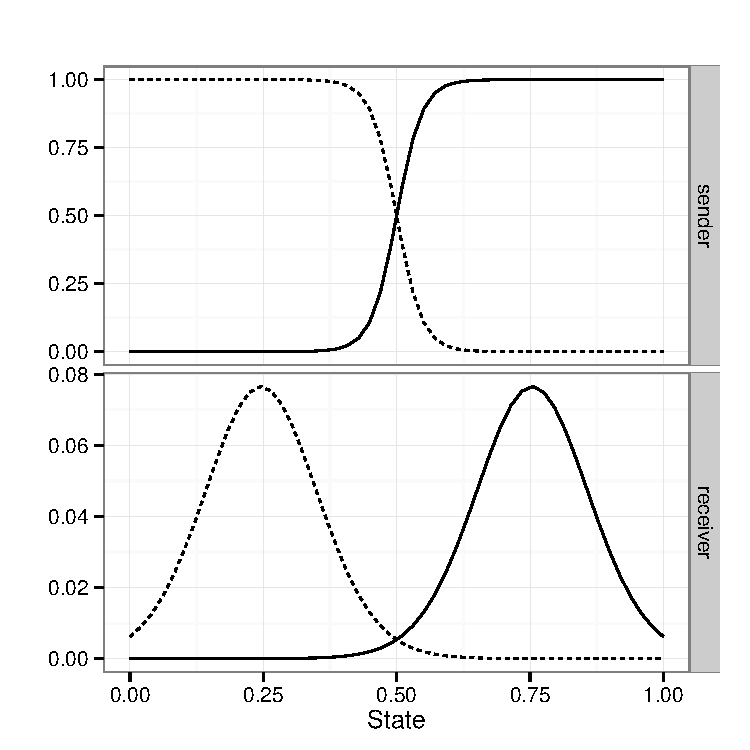
\includegraphics[width=\textwidth]{plots/exampleStratQRE_tolerance05.pdf}
    \caption{$\ns = 90$, $\lambda = 15$, $\toler = 0.5$}
    \label{fig:exampleQRE_stratsA}
  \end{subfigure}
  \hfill
  \begin{subfigure}[]{0.45\textwidth}
    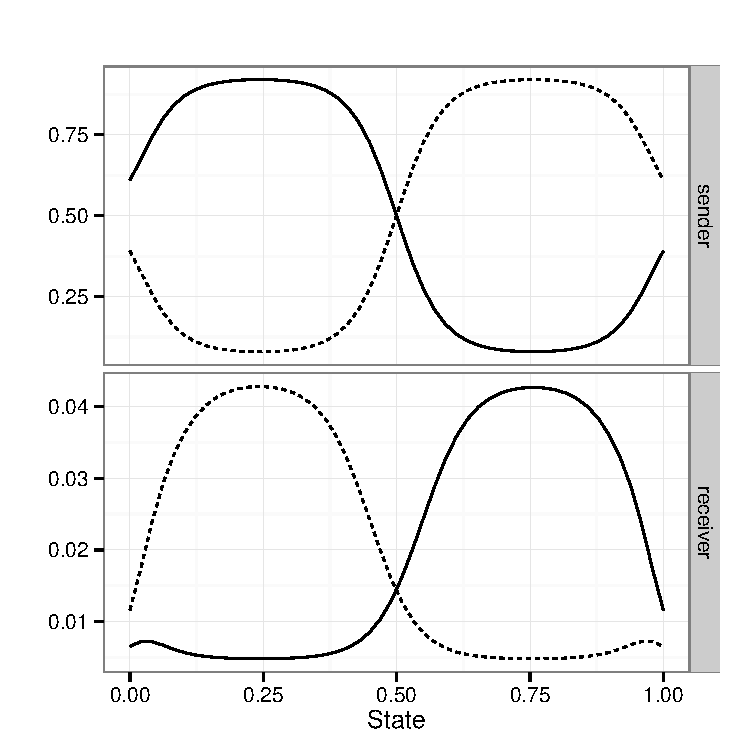
\includegraphics[width=\textwidth]{plots/exampleStratQRE_tolerance005.pdf}
    \caption{$\ns = 90$, $\lambda = 15$, $\toler = 0.05$}
    \label{fig:exampleQRE_stratsB}
  \end{subfigure}

  \caption{Examples of vague quantal response equilibria.}
  \label{fig:exampleQREs}
\end{figure}


But not all quantal response equilibria are equally plausible.
%, and the
%ones that are not suggest that it is less natural to think of
%vagueness as arising from errors in the computation or maximization of
%expected utility than that it arises from confusion of similar states
To see what the problem is, consider
Figure~\ref{fig:exampleQRE_stratsB}, which is the quantal response
equilibrium for a game with lower tolerance $\toler = 0.05$. Unlike
what evolves under \rdd in this case, sender strategies have vague
boundaries also towards the end of the unit intervals. Technically,
this is because quantal responses equalize message use far away from
the ``prototypical'' interpretation, not just in-between categories,
so to speak. This, in turn, is because quantal responses introduce
noise into the decision making at the level of computing or maximizing
expected utility of choices.

That this is problematic shows even more clearly in a case where
the state space is intuitively unbounded, as for instance for the
property ``tall.'' If the usual interpretation of a ``tall man'' peaks
at around, say, 195cm then when meeting a giant of $n$ meters, senders
would, according to the quantal response approach, be ever more
inclined to describe the giant indifferently as either ``tall'' or
``short'' the larger $n$ gets. This is because, as the distance from
the prototype increases for larger $n$, the difference between the
expected utilities of saying ``short'' or ``tall'' will converge to
zero. 
%Whence that the quantal response approach would predict that
%senders would grow indifferent between choice of antonyms as $n$
%grows, which seems weird. 

Admittedly, this argument hinges on the choice of utility
function. Still, to the extent that the utility functions we chose are
reasonable---and we think they are very reasonable---the case
suggests that quantal responses alone are not a good model for why
linguistic categories are vague. With respect to this issue, perceptual
confusion of similar states produces more intuitive predictions. What
is more plausible, though, is that both perceptual confusion \emph{and}
computational errors in maximizing expected utility play a role in
making vague categorization a pervasive feature of natural language
meaning. Perhaps even further factors, such as limited observations,
imperfect memory, and more, should be considered in order to form
a more complete understanding of the phenomenon of vagueness.

%%%%%%%%%%%%%%%%%%%%%%%%%%%%%%%%%%%%%%%%%%%%%%%%%%
%%%%%%%%%%%%%%%%%%%%%%%%%%%%%%%%%%%%%%%%%%%%%%%%%%

\section{Conclusions}
\label{sec:conclusions}

Vagueness is a pervasive but seemingly non-disruptive feature of
natural communication and classification systems. From an evolutionary
point of view, the challenge arises to explain how vagueness can
persist under selective pressure for precision. This is foremost a
technical challenge, probing for the possibility of integrating into a
consistent model forces that lead to vagueness and forces that lead
to efficient information transfer. This paper proposed one such model
in the context of sim-max games and explored some of its consequences.

We introduced the replicator diffusion dynamic as a special case of
the replicator mutator dynamic. The \rdd incorporates a special kind
of stochastic mutation due to differential confusability of similar
states. Based on data from numerical simulations, we demonstrated that
the inclusion of mild levels of stochastic confusability of states
does not undermine the possibility of evolving relatively successful
signaling strategies. On the contrary, strategies that evolved under
mild diffusion induce a highly regular and systematic category
structure that shows the signs of vagueness as desired. There might
even be a higher-order benefit to the presence of imprecision, in that
it can accelerate convergence to optimal categorization, by preventing
evolutionary paths to stay near inefficient non-convex strategies for
a long time. Diffusion thus also unifies and regularizes evolutionary
outcomes in such a way that sub-optimal categorization is avoided in
short-term trajectories.


%%%%%%%%%%%%%%%%%%%%%%%%%%%%%%%%%%%%%%%%%%%%%%%%%%
%%%%%%%%%%%%%%%%%%%%%%%%%%%%%%%%%%%%%%%%%%%%%%%%%%

\appendix

\section{Proof of Theorem}
\label{sec:proofs}

\begin{proof}[Part (i).]
  Fix $\Smixed$ and $\Sstrat = G(\Smixed)$. Look first at the rhs of
  the consequent:
  \begin{align*}
    \Diff_C(\Sstrat)(\messg_y \probbar \state_x) & =  \sum_{\state_l} C_{xl}
    \cdot \Sstrat(\messg_y \probbar \state_l) && \text{(by Equation~(\ref{eq:confusion-function}))} \\
    & =  \sum_{\state_l} C_{xl}
    \cdot  \sum_{\Spure_i(\state_l) = \messg_y} \Smixed_i && \text{(by Equation~(\ref{eq:CorrespondenceBehavioralMixed}))} \\
    & = \sum_{\state_l}
    \sum_{\Spure_i(\state_l) = \messg_y} \Smixed_i \cdot C_{xl}\,.
  \end{align*}
  Next consider the lhs of the consequent:
  \begin{align*}
    G(\Mutate_{Q^C}(\Smixed))(\messg_y \probbar \state_x) & =
    \sum_{\Spure_i(\state_x)=\messg_y} \Mutate_{Q^C}(\Smixed_i) &&
    \text{(by Equation~(\ref{eq:CorrespondenceBehavioralMixed}))} \\
    & = \sum_{\Spure_i(\state_x)=\messg_y} \sum_{\Spure_j}
    \Smixed_j \cdot Q^C_{ji} &&
    \text{(by Equation~(\ref{eq:Mutation}))} \\
    & = \sum_{\Spure_i(\state_x)=\messg_y} \sum_{\Spure_j}
    \Smixed_j \cdot \prod_{\state_l} \sum_{\state_m \in
      \Spure_j^{-1}(\Spure_i(\state_l))} C_{lm} &&
    \text{(by Equation~(\ref{eq:construction-sen}))} \\
    & = \sum_{\Spure_j} \Smixed_j \cdot
    \sum_{\Spure_i(\state_x)=\messg_y} \prod_{\state_l}
    \sum_{\state_m \in \Spure_j^{-1}(\Spure_i(\state_l))} C_{lm}
  \end{align*}
  To simplify this further we look at a fixed $\Spure_j$ and consider
  the term: 
  \begin{align}
    \label{eq:term}
    \sum_{\Spure_i(\state_x)=\messg_y} \prod_{\state_l} \sum_{\state_m
      \in \Spure_j^{-1}(\Spure_i(\state_l))} C_{lm}\,.
  \end{align}
  Let $Y$ be the row-stochastic matrix with $Y_{kl} = \sum_{\state_m
    \in \Spure_j^{-1}(\messg_l)} C_{km}$. Every pure sender strategy
  maps each state $\state_k$ onto exactly one $Y_{kl}$. If we quantify
  over all pure strategies, we essentially look at each such
  mapping. Term (\ref{eq:term}) above sums over all pure strategies
  that map $\state_k$ onto $\messg_y$. The above term then sums over
  all products whose factors are tuples in $\times_{k>2} \set{y
    \setbar \exists l \mycolon y = Y_{kl}}$. So term (\ref{eq:term})
  expands to (where $e = \card{\States}$ and $d=\card{\Messgs}$):
  \begin{align*}
    & (Y_{11} \cdot Y_{21} \cdot Y_{31} \cdot \ldots \cdot Y_{e1}) +
    (Y_{11} \cdot Y_{21} \cdot Y_{31} \cdot \ldots \cdot Y_{e2}) + 
    \dots \\
    & + (Y_{11} \cdot Y_{2d} \cdot
    Y_{3d} \cdot \ldots \cdot
    Y_{ed}) 
  \end{align*}
  But since $Y$ is a row-stochastic matrix, this simplifies to
  $Y_{xy}$. Continuing the derivation with this:
  \begin{align*}
    G(\Mutate_{Q^C}(\Smixed))(\messg_y \probbar \state_x) 
    & = \sum_{\Spure_j} \Smixed_j \cdot
    \sum_{\state_l \in \Spure_j^{-1}(\messg_y)} C_{xl} \\
    & = \sum_{\Spure_j} \sum_{\state_l \in \Spure_j^{-1}(\messg_y)} \Smixed_j \cdot
     C_{xl} \\
     & = \sum_{\state_l}
    \sum_{\Spure_i(\state_l) = \messg_y} \Smixed_i \cdot C_{xl}\,.
  \end{align*}

\end{proof}

\begin{proof}[Part (ii).]
  Fix $\Rmixed$ and $\Rstrat = G(\Rmixed)$. The rhs of the consequent
  expands to:
  \begin{align*}
    \Diff_C(\Rstrat)(\state_x \probbar \messg_y) & = \sum_{\state_j}
    \sum_{i \in \set{k \setbar \Rpure_k(\messg_y) = \state_x}}
    \Rmixed_i \cdot C_{jx} && \text{(by Equation~(\ref{eq:confusion-function}))} \\
    & = \sum_{\Rpure_i} \sum_{j \in \set{k \setbar \Rpure_i(\messg_y) = \state_j}}
    \Rmixed_i \cdot C_{jx} \\
    & = \sum_{\Rpure_i} \Rmixed_i \cdot C_{\Rpure_i(\messg_y)x} \,.
  \end{align*}
  The rhs expands to (by Equations~(\ref{eq:CorrespondenceBehavioralMixed}),
  (\ref{eq:Mutation}) and (\ref{eq:construction-rec})):
  \begin{align*}
    G(\Mutate_{R^C}(\Rmixed))(\state_x \probbar \messg_y) & = \sum_{\Rpure_i}
    \Rmixed_i \cdot \sum_{j \in \set{j \setbar \Rpure_k(\messg_y) =
        \state_x}} 
    \prod_{\messg} C_{\Rpure_i(\messg)\Rpure_j(\messg)} \,.
  \end{align*}
  Without loss of generality, assume that $x=y=1$, and fix
  $\card{M}=d$ and let $e$ be the number of pure receiver
  strategies. Then the last term can be rewritten as:
  \begin{align*}
    & = \sum_{i}
    \Rmixed_i \cdot ( C_{\Rpure_i(\messg_1)1} \cdot
      C_{\Rpure_i(\messg_2)\Rpure_1(\messg_2)} \cdot \ldots \cdot
      C_{\Rpure_i(\messg_d)\Rpure_1(\messg_d)} + \ldots  \\
      & \textcolor{white}{ = \sum_{i}
    \Rmixed_i  (}  +  C_{\Rpure_i(\messg_1)1} \cdot
      C_{\Rpure_i(\messg_2)\Rpure_2(\messg_2)} \cdot \ldots \cdot
      C_{\Rpure_i(\messg_d)\Rpure_2(\messg_d)} + \ldots  \\
      & \textcolor{white}{ = \sum_{i}
    \Rmixed_i  (}  + C_{\Rpure_i(\messg_1)1} \cdot
      C_{\Rpure_i(\messg_2)\Rpure_e(\messg_2)} \cdot \ldots \cdot
      C_{\Rpure_i(\messg_d)\Rpure_e(\messg_d)}) ) \,.
  \end{align*}
  For every messages $\messg_l$, $C_{\Rpure_i(\messg_l)}$ is a stochastic
  vector. For $l>1$, all elements of these vectors appear equally
  often. But that means that these cancel out. What remains is:
  \begin{align*}
    & = \sum_{\Rpure_i} \Rmixed_i \cdot C_{\Rpure_i(\messg_y)x} \,.
  \end{align*}
\end{proof}


%%%%%%%%%%%%%%%%%%%%%%%%%%%%%%%%%%%%%%%%%%%%%%%%%%
%%%%%%%%%%%%%%%%%%%%%%%%%%%%%%%%%%%%%%%%%%%%%%%%%%

\printbibliography[heading=bibintoc]

\end{document}
